

%% Just temporary
\tableofcontents

\section{Introduction}

%%Hardware defines the environment within which software operates.  

Software development is, in some ways, like natural 
evolution.  Every piece of software has its niche:
the environmental conditions within which it can be
used.  Within this niche it will grow and change and 
perhaps expand to nearby niches.
%%
Some niches are very large (for example, commercial PCs), some are
tiny (a newly developed humanoid).  In this paper, we are concerned
about how robotics researchers can avoid being caught in a tiny
niche, and how to prevent ``genetic isolation'' from setting in,
where software development is slow and cut-off from the mainstream.
We want to find a way to avoid this trip, without sacrificing
the freedom to radically change our hardware, a freedom that
will be crucial in ``bleeding-edge'' research for years to come.

Our motivation comes from the condition of humanoid robotics 
research, but most of this paper is not specific to that field.
%
We think it is relevant to any small research group, either academic or
industrial, who wishes to develop novel robots (as opposed to 
build applications on existing robots).  We want to maximize the 
reach of such research groups.


%Robots with unusual hardware can find themselves initially bereft of
%software, until adaptation occurs.  Therefore robots that take
%advantage of novel hardware may require significant software effort.


%Any given piece of software can operate in a certain set of 
%environments.  Every new robot is a new environment, with some
%overlap with existing ones.  Some software will run there,
%some will not.

In terms of software, robotic platforms can be quite ``genetically
isolated'' from the mainstream population of PCs.  

Research groups that all use a specific robot (Khepera, Pioneer, AIBO,
...) often form a natural software community.  But each alone is 
a small subset of robotics.

Groups developing new robots face obstacles.  There are big barriers
to software collaboration: differences in sensors, actuators, and
bodies; differences in processors, operating systems, libraries,
frameworks, languages, compilers.

Computer science and PCs operate in a world that has been at least
partially commodified; research groups in CS do not have to 
reinvent the operating system for every project they undertake.

Robot software development is like computer software development,
only more so.

Software development for humanoid robots is somewhat of a back-water.
Although it is a topic that excites the public imagination, the
actual resources devoted worldwide are quite low.  The Japanese
government and car manufacturers have invested in some high-profile
projects...


%Humanoid robotics is our passion, but in the grand scheme
%of world-wide software development 


%Big companies built on OSS (e.g. Google)



\begin{figure}
\centerline{
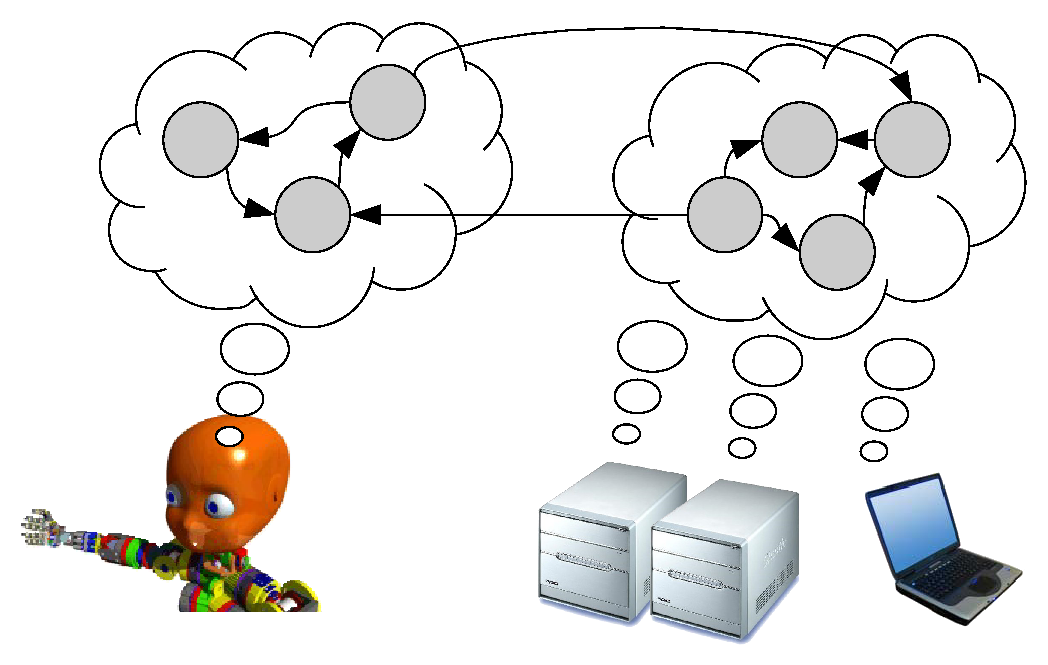
\includegraphics[width=8cm]{fig-nethead}
}
\caption{
%
Basic robot model.  We assume a set of computers, some of which may be
on the robot, some of which may not be.  We assume that the computers
are diverse: they may have different devices, operating systems,
processors, and the programs they run may use different languages,
libraries, etc.  We nevertheless require that threads within processes
on any of these computers be able to communicate easily with each other.
This communication, ideally, should fit well with basic UNIX 
tools and concepts (although we do not assume the operating systems
in use are UNIX-based).
%
%
%
(specific iCub example given later).
%
}
\end{figure}








\section{A software ecology}

Many robot projects are ``black holes'', in terms of software.  A lot
of software gets sucked in, but very little comes out.  Once a piece
of software has been adapted to a particular robot, it takes a lot
of work to extricate it again and apply it to another.

Obviously the answer to this problem is modularity.  So there are 
now many architectures/frameworks/... for modular robot systems.
The prime concern for any such system should be that it is not
a ``black hole'' -- that once a piece of software has been adapted
to a particular framework, it takes a lot of work to extricate it
again and apply it to another.  That would be a bit self-defeating.

We study YARP from this perspective.  How sticky is resultant user
code to the robot and to the framework itself?


The way parts interact can last longer than the parts themselves.
Long-lived software is like the Ship of Theseus -- the mast gets replaced,
the planks get replaced, over time everything may get replaced (``paradox
of identity'').


\subsection{Free and Open Source}

Useful, more malleable.

Has the pragmatic benefit that a user of the software can
modify and integrate it to their hearts content without the 
pain of dealing with opaque binaries.

Has the revolutionary benefit that the user is not trapped in the role
of being a ``consumer'' of software, but can also be a publisher of
the changes, additions, and integrative work they do in an effective
form.  This is achieved by explicitly granting far more rights to
users than they have under the law of most countries, contrasting with
agreeably with the formerly more common practice of attempting to
minimize user rights.  These rights are typically granted
conditionally; a user may only make use of these extended rights if
(for example) distributed code is always available in its most useful
original (source) form, with compatible freedoms attached to it.  This
condition seeks to balance freedoms of individuals versus benefit to
the group.  The existence of code in usable form with freedoms 
attached can benefit many people;

The freedom to distribute code in obscure (compiled) forms



Split between people who emphasize pragmatic concerns and those
who emphasize freedom.  Just cite the issue, no need to revisit
it here.




\subsection{C/C++}

very portable (especially C), though lots of details.

but compile process?  varies a lot. autobuild tools
(autoconf/automake).  and also CMAKE.

CMAKE:

Open-source, deals well with various IDEs and command-line development.

Not as familiar as autoconf/automake/... etc.

Has the excellent property of being simpler than making Makefiles
or configuring a project, when external libraries are involved.

The big downside is that the language is unfamiliar and a bit ugly.
It is simple and well-documented, but quirky.  An alternative with
some similar properties, scons, uses python instead.  The ant system
uses with java also seems cleaner.  However, it gets the job
done, and has the huge advantage of not being dependent on an
external language being installed.

CMake is free and open-source, with a healthy community of 
developers.


SWIG:

ACE:


\subsection{Repositories}

sourceforge.  debian.

RANT FOLLOWS

The literature of a research community both expresses its ideas, and
aids in their evolution

Published ideas are read, evaluated, and built upon

Useful advances get published

Publication of software can speed progress

Facilitates evaluating and comparing approaches

Brings new research topics into reach

Publish or perish!

REPEATED RANT FOLLOWS

As a research community, we both read and produce papers, building on
each others' work.

We also both acquire and produce software

Our software tends to die with our projects

Sad!  Software collaboration speeds things up

Research groups that all use a specific robot (Khepera, Pioneer, AIBO,
...) often form a natural software community

But each alone is a small subset of robotics

Groups developing new robots face obstacles

Differences in sensors, actuators, bodies...

Differences in processors, operating systems, libraries, frameworks,
languages, compilers...

Big barriers to software collaboration




\subsection{Modularity}

Constant hardware flux

Parts change rapidly

Interfaces change slowly

Lots of software grew and evolved alongside the changing hardware

Parts change rapidly

Interfaces change slowly

``Modularity'' is rewarded


The way parts interact can last longer than the parts themselves

E.g. an eternal broom

replace broom head

replace broom handle


Long-lived software is like the Ship of Theseus

The mast gets replaced

The planks get replaced

Over time, everything may get replaced

In philosophy, this is a ``paradox of identity''

For us, it's just our job


The opposite of a modular system is a coupled one.

In a ``coupled'' system, changes in one part trigger changes in another.

Coupling leads to complexity

Complexity leads to confusion

Confusion leads to suffering

This is the path to the Dark Side

Robot software is notoriously hardware-specific and task-specific

Both hardware and target tasks change quickly, even within the
lifetime of one project

Our humanoid robots are far more complex than one person can build and
maintain, both in terms of hardware and software

They need to be modular





\section{YARP Basics}


The sad fate of most robot software

Modularity in robotics

YARP: Yet Another Robot Platform

Excising communication ``plumbing'' from code

Excising device dependencies from code



YARP is an open-source software library  for humanoid robotics

History

An MIT / LIRA-Lab collaboration

Born on Kismet, grew on COG

With a major overhaul, now used by RobotCub consortium

Exists as an independent open source project

C++ source code



\subsection{What is YARP for}


Factor out details of data flow between programs from program source code

Data flow is very specific to robot platform, experimental setup,
network layout, communication protocol, etc.

Useful to keep ``algorithm'' and ``plumbing'' separate

Factor out details of devices used by programs from program source code

The devices can then be replaced over time by comparable alternatives;
code can be used in other systems




\subsection{Two views of a robot}

From a software perspective, it is natural to consider a robot
as a bundle of devices (sensors and actuators) that can be
queried and controlled via whatever interfaces they provide.
In YARP, we call this the ``device view'' of the robot.

Interfaces to devices can be very idiosyncratic.  Some
classes of devices (such as certain classes of camera) have become
commoditized, and have relatively standard interfaces, leaving the
user with considerable freedom in how those interfaces are used in
software.  Other devices may be bundled with vendor-supplied software,
without much freedom for the user to avoid dependencies or work around
flaws.  This is understandable behavior on the part of a company,
since decoupling their hardware and software could lead to more rapid
competition and eventually commoditization, requiring rapid adjustment
of business model in order to maintain competitiveness.  However,
it can leave users of hardware in a bit of a bind.


YARP offers two almost equivalent views of a robot.


A set of ports to which you can connect and get data or send commands
(port view).

A set of devices which you can control or query according to a choice
of interfaces (device view).

The local device view: you are responsible for configuring and starting devices

The remote device view: configuration and starting-up/shutting-down is
packaged with the robot

